\chapter{Introducción específica} % Main chapter title

\label{Chapter2}

%----------------------------------------------------------------------------------------
%	SECTION 1
%----------------------------------------------------------------------------------------
Este capítulo explica las tecnologías aplicadas en el desarrollo de la pantalla gigante fullcolor. Se presentan los requerimientos identificados al iniciar el trabajo para cumplir con los objetivos.
\section{Matriz de LEDs}
La matriz de LEDs es un conjunto o arreglo de LEDs  bidimensional donde los cátodos se unen en filas y los ánodos se unen en columnas. Existen numerosos métodos para controlar las matrices de LEDs, para desarrollar este proyecto se seleccionó el método de multiplexación debido a su bajo uso de recursos en comparación a controlar los LEDs de manera individual \citep{CONCEPTOMATRIZ}.
\subsection{Multiplexación de una Matriz de LEDs }
La multiplexación es una técnica de control de matrices LED en donde se habilita una fila de LEDs a la vez y las columnas se habilitan de acuerdo a el pictograma que se desea mostrar en la matriz de LEDs, luego se habilita las siguientes filas repitiendo el proceso anterior, una vez terminado el proceso para todas las filas de LEDs se procede a comenzar el ciclo nuevamente, la frecuencia del ciclo debe ser superior a 30 Hz para evitar que ojo humano detecte el parpadeo \citep{MULTIPLEXADO}.

En la figura \ref{fig:matrizled} se puede observar una matriz de LEDs de cuatro filas por cuatro columnas, para mostrar el pictograma se siguen los siguientes pasos:

\begin{enumerate}
\item Se habilita la fila T3.
\item Se habilita la columna N1.
\item Se espera un momento.
\item Se habilita la fila T2.
\item Se habilita las columnas N1, N2 y N3.
\item Se espera un momento.UDP
\item Se habilita la fila T1.
\item No se habilita ninguna columna.
\item Se espera un momento.
\item Se habilita la fila T0.
\item No se habilita ninguna columna.
\item Se espera un momento.
\item Se repite el ciclo desde el paso uno.
\end{enumerate}


\begin{figure}[htpb]
	\centering
	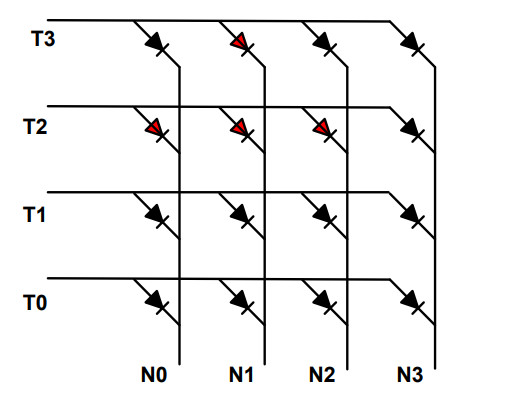
\includegraphics[scale=0.5]{Figures/ledmatrix.jpg} 
	\caption{Matriz de LEDs \protect\footnotemark.}
	\label{fig:matrizled}
\end{figure}

\footnotetext{Imagen tomada de \url{https://web.stanford.edu/class/archive/engr/engr40m.1178/slides_sp17/lecture10.pdf}}

La manera de habilitar las filas es a través de MOSFET canal P y las columnas se habilitan a través de drivers de LEDs.
 
 

%\https://bibdigital.epn.edu.ec/bitstream/15000/9935/1/SISTEMA%20DE%20INFORMACION%20VISUAL.pdf




\subsection{Driver de led MBI5051}
El driver que se eligió para habilitar las columnas de LEDs fue el driver MBI5051, este driver fue diseñado para ser usado en pantallas exteriores de vídeo, las características del driver se muestran en la tabla \ref{tab:driverled}.

\begin{table}[h]
\centering
\caption[Características MBI5051]{Características del driver MBI5051 \protect\footnotemark.}
\begin{tabular}{l c c}
\toprule
\textbf{Especificaciones}& \textbf{Detalles}\\
\midrule 

Voltaje alimentación & 3.0V-5.5V\\
Canales de corriente constante & 16\\
Rango de corriente constante por canal & 2 a 45 mA\\
Profundidad de color & 14 o 16 bits\\
Máxima frecuencia de reloj & 30 Mhz\\

\bottomrule
\hline
\end{tabular}
\label{tab:driverled}
\end{table}

\footnotetext{Referencia tomada de \url{https://www.neumueller.com/datenblatt/macroblock/MBI5051\%20Datenblatt\%20-\%20Datasheet.pdf}}



\section{ Plataforma de desarrollo DE1SoC}
Se eligió la plataforma DE1SoC debido a que cumple con los requerimientos, otra de las razones para escoger esta plataforma fue que dentro de la empresa se la ha usado para el desarrollo de proyectos previos, lo cual ahorró mucho tiempo de aprendizaje. Las especificaciones de la plataforma se muestran en la tabla \ref{tab:DE1SOCTABLA}.

\begin{table}[h]
\centering
\caption[Especificaciones DE1SoC]{Especificaciones DE1SoC \protect\footnotemark.}
\begin{tabular}{l c c}
\toprule
\textbf{Especificaciones}& \textbf{Detalles}\\
\midrule 


Procesador & ARM CORTEX A9\\
HPS SDRAM & 1GB DDR3\\
FPGA SDRAM & 64MB SDRAM\\
UART & UART a USB\\
FLASH & EPCS128\\
Puertos USB & 2\\
Pines GPIO & 36X2\\
Ethernet & 1 Gigabit\\


\bottomrule
\hline
\end{tabular}
\label{tab:DE1SOCTABLA}
\end{table}

\footnotetext{Referencia tomada de \url{https://www.terasic.com.tw/cgi-bin/page/archive.pl?Language=English&CategoryNo=205&No=836&PartNo=1}}

La plataforma cuenta con un procesador y un FPGA dentro del mismo CHIP como se puede observar en la figura  \ref{fig:DE1BLOCK}. El FPGA fue usado para controlar la matriz de LEDs debido a su capacidad de manejar varias salidas GPIO en paralelo y el procesador fue usado para manejar las comunicaciones.

\begin{figure}[htpb]
	\centering
	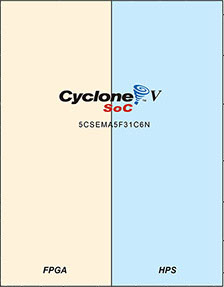
\includegraphics[scale=0.4]{Figures/fpgablock.jpg}  
	\caption{Diagrama de bloques DE1-SoC \protect\footnotemark.}
	\label{fig:DE1BLOCK}
\end{figure}

\footnotetext{Referencia tomada de \url{https://www.terasic.com.tw/attachment/archive/836/image/image_77_thumb.jpg}}


\section{Lenguaje descriptor de hardware}


El lenguaje seleccionado para describir el hardware fue VERILOG. Los diseñadores de VERILOG tuvieron como objetivo que la sintaxis sea similar a la del lenguaje C para que fuera aceptada por los ingenieros. El lenguaje posee un preprocesador similar al lenguaje C ademas de compartir palabras reservadas de control. A pesar de tener una sintaxis muy similar a C difiere en la definición de constantes requiere la longitud de bits, no tiene estructuras, apuntadores o funciones recursivas. 

No todas las sentencias del lenguaje son sintetizables. Si las sentencias de todos los modulos son sintetizables, se pueden convertir en una lista de nodos que describe los componentes básicos. "La lista de nodos puede entonces ser transformada en una forma describiendo las celdas estándar de un circuito integrado, por ejemplo ASIC, o una cadena de bits para un dispositivo de lógica programable (PLD) como puede ser una FPGA o un CPLD"  \citep{WIKIVERILOG}.




\section{Protocolos de comunicaciones UDP}
UDP es el acrónimo de protocolo de datagrama de usuario, UDP es un protocolo de comunicaciones que pertenece a la capa de transporte, este protocolo permite la transmisión de datos sin conexión preliminar, tampoco tiene confirmación de recepción. Se usa en aplicaciones en donde el intercambio de paquetes de la conexión o desconexión son mayores a la información transmitida o en aplicaciones de transmisión de audio y vídeo en tiempo real debido a que retransmitir agregaría retardos \citep{WIKIUDP}.


\section{Sistema operativo de propósito general para embebidos}

El sistema operativo que se utilizó en el desarrollo de este proyecto fue Linux embebido.Linux embebido se refiere al uso del núcleo Linux  en un sistema embebido combinado con un conjunto de utilidades de software libre. 
%\https://es.wikipedia.org/wiki/Linux_embebido
El núcleo de Linux o \textit{kernel} es la interfaz entre el hardware de un PC y sus procesos \citep{KERNEL}. Las tareas que realiza el \textit{kernel} son:

\begin{itemize}
\item Gestión de memoria: control de cantidad de memoria y locación de la misma.
\item Gestión de procesos: administra que procesos usan la CPU y cuanto tiempo.
\item Controladores de dispositivos: interfaz entre hardware y procesos.
\item Seguridad y llamadas de sistema: recibe solicitud de servicio desde procesos. 
\end{itemize}


\subsection{Samba}
SAMBA es una aplicación que permite que las carpetas compartidas dentro del sistema operativo Linux, Mac OS X o Unix  puedan ser abiertas desde un computador con sistema operativo Windows \citep{WIKISAMBA}.

\subsection{Servicio de Linux}

Los servicios son programas que se ejecutan fuera de la vista y control del usuario ya que no cuentan con interfaz gráfica. Existe algunos servicios que son muy importantes para el funcionamiento del sistema operativo.
En sistemas UNIX o LINUX, los servicios son conocidos como demonios \citep{SERVICIO}.

\subsection{SYSTEMD}

SYSTEMD es un software de administración de sistemas y servicios, el objetivo principal de este software es que la configuración y comportamiento de los servicios sea el mismo en todas las distribuciones de Linux. Se puede utilizar SYSTEMD para realizar configuraciones al iniciar el sistema \citep{REFSYSTEMD}.

\subsection{Bash script}
BASH es un interprete de comandos. Está presente en una amplia variedad de sistemas operativos y es el interprete de comandos por defecto en los sistemas GNU/LINUX \citep{BASH}. 


BASH SCRIPT es un texto plano que contiene una serie de comandos. Esta lista de comandos es una mezcla de comandos que son comúnmente escritos por medio de la consola \citep{BASHSCRIPT}. El uso de bash scripting permite:

\begin{itemize}
\item Automatizar acciones repetitivas.
\item Mejor experiencia de usuario debido a lo anterior.
\item Ofrece herramientas al administrador para que el sistema operativo sea más ágil y automático.
\end{itemize}

\section{Requerimientos}
En esta sección se indican los requerimientos que fueron propuestos para el proyecto.

\subsection{Grupos de requerimientos asociados con hardware}

Tarjeta de distribución:
\begin{itemize}
\item Debe tener conectores de entrada IDC40 con la misma distribución de pines usados en las salidas GPIO de la board DE1-SoC.
\item Debe cambiar los niveles de voltaje de 3.3 v a 5 v de todas las entradas. 
\item Debe manejar señales de una frecuencia de entre 5 Mhz a 10 Mhz.
\item Debe tener conectores de salida IDC16 compatibles con la distribución de pines usados en las matrices de leds.
\end{itemize}
Matriz de leds:
\begin{itemize}
\item Debe tener un conector de entrada y un conector de salida IDC16.
\item Debe ser capaz de manejar frecuencias de hasta 10 Mhz.
\item Debe tener drivers de leds con escala de grises de 16 bits.
\item Debe tener 16 leds de alto por 16 leds de ancho.
\item Debe ser capaz de pasar la información de la entrada a la salida.
\item Debe poder realizarse control por barrido. 
\item La pantalla tendrá una dimensión de 400 pixeles de largo por 96 pixeles máximo.
\end{itemize}

\subsection{Grupos de requerimientos asociados con el software}

Sistema operativo:
\begin{itemize}
\item Debe ser capaz de inicial y restablecer el programa del procesador automáticamente.
\item Debe ser capaz de conectarse a la red lan. 
\item Debe ser capaz de compartir una carpeta para el proceso de cargado de imágenes.
\item Almacenamiento interno de hasta 500 imágenes.
\end{itemize}

Firmware procesador:
\begin{itemize}
\item Debe ser capaz de leer las imágenes que se encuentran en la carpeta compartida.
\item Debe ser capaz de escribir en una  memoria ram accesible para el FPGA  las imágenes a ser desplegadas.
\item Debe administrar el despliegue de las imágenes por medio de un archivo externo que sea enviado desde la central de control.
\end{itemize}
\subsection{Grupos de requerimientos asociados al FPGA}
FPGA:
\begin{itemize}
\item El FPGA debe ser capaz de manejar a la pantalla led a una frecuencia de  30 hz.
\item Debe leer la información del los leds de una memoria ram que comparta con el procesador.
\item Debe manejar los drivers de led a través de una máquina de estado finita.   
\end{itemize}